%*******************************************************************************
%*********************************** First Chapter *****************************
%*******************************************************************************

\chapter{Introduction}
\label{chap1:sec:introduction}

Vision is probably the most important of all senses that humans possess. Our society is built on having the ability to see. For example, if we want to cross a street, thick colored stripes on the road and signs above our heads indicate where the cross walk is located in order for us to cross the street appropriately. Another example is how we use text to communicate with each other, where messages that we read and write consist of sequences of symbols that are structured into words of some specific language. Furthermore, visuals are used frequently in education to help students comprehend new information and concepts. Basically, many everyday tasks such as traveling, communication, and learning become more convenient with normal vision. 

%Vision is probably the most important of all senses that humans possess. Our society is built on having this ability. For example, if we would like to cross a street, there are thick colored stripes on the road or signs above head height that indicate where the cross walk is located such that we can cross the street in an appropriate way. Another example is how we use text to communicate with each other, where words and sentences are composed by structured sequences of symbols that constitute a specific language. 
%%Much media and entertainment, such as computers, television, and theatres, with performers acting various scenes requires our capability to see. 
%Furthermore, it has been shown that learning from both images and text can improve comprehension over learning from text only~\cite{eitel2013picture, hibbing2003picture}. Possessing normal vision capabilities basically make everyday tasks easier when it comes to reaching destinations in the world, communicating with other people, and learning new concepts.  

Millions of people have visual impairments that cannot be treated with correctable eyewear~\cite{bourne2021trends}. To enhance the mobility of visually impaired (VI) people, there exist various kinds of assistive tools, such as screen readers and Braille typewriting machines, for supporting them with receiving information and communicating through text. 
More recently, several assistive vision technologies have emerged in the form of mobile phone applications~\cite{microsoft2017seeing, clary2018lookout,cloudsight2013taptapsee, envision2018app,bemyeyes2017be, aira2017aira} and wearable devices~\cite{orcam2019myeye, envision2020glasses,caraiman2017soundofvision}. Furthermore, several works in computer vision research has been specifically focused developing methods for assisting VI people with, e.g., visual recognition~\cite{ahmetovic2020recog, jafri2014computer, kacorri2017teachable,gurari2018vizwiz,massiceti2021orbit,kacorri2017people,lee2019hands,lee2019revisiting} and wayfinding~\cite{coughlan2009functional, kacorri2018environmental, loomis2020assisting,szpiro2016finding,tian2013toward,lee2020pedestrian}. 

%However, there are unfortunately people who partly or fully lack the ability to see. In 2020, it was estimated that 43.3 million people who were considered blind and 295 million people having a moderate or severe visual impairment in the world~\cite{bourne2021trends}. To enhance the mobility of visually impaired (VI) people, there exist various kinds of assistive devices and tools, such as screen readers and Braille typewriter machines, for supporting them with receiving information and communicating through text. More recently, several computer vision-based assistive vision tools have emerged in the form of wearable devices and mobile applications for helping VIs with tasks where visual information is a must, e.g., object recognition~\cite{ahmetovic2020recog, jafri2014computer, kacorri2017teachable} and wayfinding in natural environments~\cite{coughlan2009functional, kacorri2018environmental, loomis2020assisting} and . 



Despite the recent advances in deep learning for computer vision~\cite{krizhevsky2012imagenet,he2016deep, redmon2017yolo9000,xu2015show,anderson2018bottom}, several challenges have been demonstrated when deploying computer vision models in real-world scenarios. For example, the models may surprisingly fail to recognize known objects appearing in new poses~\cite{alcorn2019strike}, lighting conditions~\cite{dai2018dark}, and geographical locations~\cite{de2019does}, models trained on images from one set of hospitals may perform poorly on image conditions from another~\cite{koh2021wilds}, and models can suffer from biases that disadvantage certain users based on their gender and ethnicity~\cite{buolamwini2018gender}. Part of the reason for these challenges is that specifying a model that can be injected with the rich complexity of the real world is difficult~\cite{szeliski2010computer}. 
To enhance their applicability in the real-world, researchers are striving for developing computer vision models that can recognize objects in detail~\cite{wei2021fine}, learn new abilities continuously~\cite{delange2021continual,parisi2019continual}, and adapt fast to new scenarios from few examples~\cite{wang2020generalizing,xian2018zero,hospedales2020meta}. Furthermore, such tasks should be possible to execute in a time-efficient and robust manner in assistive vision devices to improve the user experience.  


%Despite the recent successes in computer vision~\cite{he2016deep, redmon2017yolo9000, xu2015show,krizhevsky2012imagenet,anderson2018bottom}, these methods can face several challenges when deployed in the real-world, which makes their recognition performance suffer. For example, it can be difficult for the methods to distinguish between similar items on a fine-grained level, such as different brands of apples and pears, as well as performing robustly in environments with noisy backgrounds and poor lighting. Part of the reason for such challenges is that it is difficult to specify a model and inject it with knowledge about the rich complexity that can exist in the real world~\cite{szeliski2010computer}.
%%Part of the reason for such challenges is that specifying a model of the visual world that has been injected with knowledge about the rich complexity that can exist in images is very difficult~\cite{szeliski2010computer}. 
%Therefore, there is a necessity for developing computer vision methods that can recognize different appearances of objects, adapt to changes of known objects, and learn what new objects look like. At the same time, these tasks should be possible to execute in a time-efficient and robust manner to enhance the user experience. 

In this thesis, we address challenges on computer vision models for recognizing objects and their fine-grained details, as well as continually adapting the models to new concepts while retaining its previously learned knowledge. 
We will continue this chapter by briefly describing visual impairments in Section \ref{chap1:sec:vision_impairments}, followed by a summary of assistive vision technologies in Section \ref{chap1:sec:assistive_vision}. Section \ref{chap1:sec:scope_of_thesis} describes the scope of the thesis, and we summarize the contributions of the included papers in Section \ref{chap1:sec:contributions}. In Section \ref{chap1:sec:outline}, we present the overall outline of this thesis. 

%In this thesis, we address challenges on robustness in fine-grained image recognition as well as how to enable computer vision methods to update themselves with new object classes to recognize. We will begin this introduction by briefly describing vision impairments in Section \ref{chap1:sec:vision_impairments}, followed by a summary of assistive vision technologies in Section \ref{chap1:sec:assistive_vision}. Then we describe the scope of the thesis in Section \ref{chap1:sec:scope_of_thesis} and summarize the contributions of the included papers in Section \ref{chap1:sec:contributions}. Finally, in Section \ref{chap1:sec:outline}, we give the outline to the rest of the contents in this thesis. 


%Vision is one of the most important senses that humans possess. It is an amazing process of how the eyes and brain translate light waves into interpreted images of our surroundings. Reflected light waves from objects are bent, or refracted, when passing through the cornea, then bent again passing through the lens and eventually hits the retina. The image is translated into impulses that travels to the brain, more specifically the occipital lobe, through the optic nerve such that the image can be interpreted. The shape of eyes affect how we things in the world are seen and kept in focus. For people with normal vision, the light waves hits the retina at the focal point where the light waves coincide. However, the eyes are longer for nearsighted eyes which moves the focal point closer to the lens such that the light waves are more spread out across the retina. For farsighted people, the eyes are shorter which moves the focal point behind the retina. Luckily, the position of the focal point can be corrected for both near- and farsighted eyes by placing a concave and convex lens respectively in front of the eyes, e.g., by using eyeglasses. However, there exist many severe cases of low vision where not even eyeglasses can help where other kinds of help is necessary for assisting the people in situations where vision is a necessity. 

%There exist many different types of aids and assistive tools for helping visually impaired people (VIP) in their daily lives. A very common aid is the white cane used for enhancing the mobility of VIPs by extending their touch to prepare the users for what is ahead of them. There also exists many electronic devices, e.g., screen readers and Braille typewriter machines, that have enabled VIPs to have near-equal opportunities for office work. More recently, several computer vision-based assistive vision tools have emerged in the form of wearable devices and mobile applications for helping with, e.g., reading printed documents and bar codes for item recognition. However, computer vision-based systems can face several challenges when deployed in the real world which makes their recognition performance suffer. Therefore, there is a necessity for developing computer vision methods that perform various kinds of recognition tasks in a robust and time-efficient manner. 

%Despite the immense successes in computer vision in recent years, why is computer vision difficult to perform in real-world settings? One part of the reason is that it is very challenging to specify a model of the visual world that has been injected with knowledge about the rich complexity that can exist in images~\cite{szeliski2010computer}. Interestingly, tasks that are seemingly simple for humans, such as the differences between apples and pears, can be difficult for computers. A popular approach for enabling computers to learn various concepts is machine learning where the computer learns a model of some phenomena from large sets of examples. The approach of learning from data and experiences has been shown across various tasks~\cite{akkaya2019solving, brown2020language, silver2016mastering} other than computer vision to be more efficient than relying on hard-coded knowledge for solving decision-making problems. However, collecting large sets of data is often time-consuming and labor-intensive which makes it challenging to deploy machine learning systems in the real-world where data is even more expensive to collect. Without overcoming the challenge of data collection, we need to develop data-efficient methods that can learn from few examples and generalize to new scenarios for enabling computer vision-based assistive vision devices to be useful for VIPs.   




\section{Visual Impairments}\label{chap1:sec:vision_impairments}

A visual impairment is defined as the decrease of an individual's ability to see from various distances~\cite{who2022international}. The conditions varies from having issues with seeing from far or near distances to blindness, i.e., complete or nearly-complete vision loss. Visual capabilities are in general assessed by measuring the visual acuity (sharpness) of seeing from some fixed distance, e.g., letters of different size on an eye chart. 
The visual acuity is measured differently based on whether near- or far-sighted VI people are being assessed. For far-sighted VI people, visual acuity is calculated by the ratio between the distance that the subject and a normal-sighted person can recognize the target object.
For near-sighted VI people, visual acuity is measured using a standardized point system defining the font size of letters that the subject can recognize~\cite{who2019world}.


%A visual impairment is defined as the decrease of one's ability to see from various distances~\cite{who2022international}. There are different types of VIs ranging from various degrees of blindness to having issues with seeing from far or near distances. The visual capabilities are in general assessed by measuring the \textit{visual acuity} (sharpness) of seeing, for example, a letter or symbol, from some fixed distance. The visual acuity measured differently based on whether near- or far-sighted VI is assessed. For far-sighted VI, the visual acuity is calculated by the ratio between the distance in which %that 
%the subject can see the item and the distance in which a normal-sighted person could recognize the item. When assessing near-sighted VI, one checks the font size of letters that the subject can see using a standardized point system for measuring the symbol size~\cite{who2019world}. %%Worth noting is that to be considered having a VI, it is taken into account whether the the vision capabilities are possible to correct with eye-glasses or contact lenses [citeation here].   

In 2020, it was estimated that 338 million people possess a moderate to severe visual impairment globally, including 43 million people that are blind~\cite{bourne2021trends}. Furthermore, the World Health Organization (WHO) have estimated that at least 2.2 billion people live with a near or distance visual impairment, where at least 1 billion cases could have been prevented or yet has to be addressed~\cite{who2019world}. The number of untreated cases is projected to be 1.7 billion people by 2050, mainly due to global population growth as well as increased aging among the populations~\cite{bourne2021trends}. 
The main causes for having vision loss are uncorrected refractive errors, untreated cataracts, age-related macular degeneration, glaucoma, diabetic retinopathy, where 90\% of such cases are preventable and treatable~\cite{steinmetz2021causes}. These causes also varies between different countries and regions with different socioeconomic status.  

%In 2020, it was estimated that 338 million people possess moderate to severe VI globally, including 43 million people that are blind~\cite{bourne2021trends}. Furthermore, the World Health Organization (WHO) have estimated that at least 2.2 billion people live with a near or distance VI, where at least 1 billion cases could have been prevented or yet has to be addressed~\cite{who2019world}. The untreated cases are projected to grow to 1.7 billion people by 2050 mainly due to population growth in the world as well as increased aging among the populations~\cite{bourne2021trends}. The leading causes for vision loss are uncorrected refractive errors, untreated cataracts, age-related macular degenerationm, glaucoma, diabetic retinopathy, where 90\% of such cases are preventable and treatable~\cite{steinmetz2021causes}. The causes for vision loss also differs between countries and areas with different incomes.  

There exists many kinds of tools for assisting VI people with everyday tasks. The white cane and guiding dogs are probably the most common tools for enhancing their mobility by preparing the user for what is present in their near surroundings. Furthermore, there are different tools for various visual recognition tasks, such as currency markers for identifying different bills in wallets, color indicators for notifying the user of the color of clothes, and labeling apparatus with Braille writing for distinguishing between similar items~\cite{srf2017vardagstips}. There also exist Braille keyboards and screen readers compatible with both computers and mobile phones for helping VI people with e.g. sending text messages and emails, surfing the web, and using calendar apps~\cite{gotesson2019challenges}. In the next section, we introduce a selection of assistive vision technologies aimed for assisting VI people with recognition of objects in their environment. 
 

%There exists several tools for assisting VI people with everyday tasks. The \textit{white cane} is probably the most common tool among VI people which is used for wayfinding to help the user anticipate what is present in their near surroundings. Also, guiding dogs are used for enhancing mobility by helping VI people to maintain a direct route, avoid obstacles, and prepares owner by stopping at %curbs and 
%stairways until they are told to proceed~\cite{manduchi2012computer}. There also exist several tools for recognition tasks. For example, currency markers are used for keeping track of different bills in wallets, color indicators can be used to tell the user of the color of clothes, and labeling apparatus are used for distinguishing between similar items. Means for communication also exists in the form of Braille keybords and screen readers that are used in both computers and mobile phones to provide nearly equal opportunities for VI people when it comes to office-related tasks. %There has been a recent emergence of various devices that are aimed to assist VI people with object recognition tasks which we will discuss next.  

%Next, we will discuss the recent emergence of various computer technologies that are aimed to assist VI people with object recognition tasks.  




%There are many different degrees of vision impairments ranging from problems with seeing from near or farther distances to blindness. Vision impairments are generally assessed by measuring the visual acuity from a fixed distance~\cite{who2019world}. In 2020, the World Health Organization (WHO) estimated that at least 2.2 billion people live with a near or distance vision impairment, wherein at least 1 billion cases the impairments could have been prevented or yet has to be addressed~\cite{who2019world}. The untreated cases are projected to grow to 1.7 billion people by 2050 mainly due to population growth and aging~\cite{bourne2021trends}. The leading causes for vision loss are uncorrected refractive errors (161 million people with distance vision loss and 510 million people with near vision loss), untreated cataracts (100 million people), age-related macular degenerationm (8.1 million), glaucoma (7.8 million), diabetic retinopathy (4.4 million) where 90\% of vision losses are preventable and treatable~\cite{steinmetz2021causes}. Furthermore, the prevalence of distance vision impairment are estimated to be four times higher in low- and middle-income regions than in high-income regions~\cite{steinmetz2021causes}.  

%Several kinds of aids and tools have been developed for VIs to facilitate their capabilities of performing everyday tasks. The so-called \textit{white cane} is by far the most common mobility tool aid which is used for navigation and helping the VI to anticipate what is in front of them while walking. Dog guides are also used for enhancing mobility by helping the VI to maintain a direct route, avoid obstacles, and stops at curbs and stairways until they are told to proceed~\cite{manduchi2012computer}. Technical devices such as screen readers and Braille keyboards have enabled VIs to have nearly equal opportunities when it comes to office-related tasks. Furthermore, eye-service clinics offer counseling and home-skills training for helping VIs with modifying their home to ensure a safe and accessible home. 

%\MK{I should mention difference between low-vision and blindness somewhere here too.}


%In Sweden, there are over 100.000 people with 




%In 2020, there were almost 600 million people with mild to severe visual impairments around the world~\cite{bourne2021trends}. 

%Describe common causes for visual impairment. What aids are there for helping them out, which will lead to assistive vision devices in the next section. 

%In a recent study made in Sweden with VIs, the challenge that most VIs are concerned about in general is mobility~\cite{stahl2018levnadsundersokning}. 

%VIPs that had to change their careers due to inaccessible apps and systems at their workplace~\cite{gotesson2019challenges, gotesson2019utmaningar}. Conclusion was that VIPs should be involved in the development and design process of such products, and that this should be included when educating User Experience (UX) designers. 


\section{Assistive Vision Technologies}\label{chap1:sec:assistive_vision} 

Cameras are used by blind people to record events and memories similarly as people with normal vision~\cite{jayant2011supporting}. Moreover, there is an urge among VI people to use their cameras for daily tasks other than recording events, such as object recognition~\cite{brady2013visual}, face recognition~\cite{zhao2018face}, and currency identification~\cite{liu2008camera}. 
In this thesis, we focus on object recognition which can be challenging in many ways without visual information. For instance, VI people may need assistance from non-visual cues indicating how to capture the whole item in the camera view~\cite{vazquez2012helping}, and also may need to point the camera towards some specific side of the object to identify details of interest to the user. These challenges have encouraged the development of technical aids that use computer vision for assisting VI people which we will cover next. 


%Cameras are used by people with VIs, including blindness, to record events and memories similarly as normal-sighted people~\cite{jayant2011supporting}. This has opened up for opportunities where VI people can use their cameras for more than recording events, for example, object recognition, document text recognition, and color identification. Object recognition has been shown to be considered an everyday challenge, where VI people would like to ask questions about objects where visual information is necessary for identification~\cite{brady2013visual}. For example, it can be very difficult to distinguish between different containers and packages that have similar shapes but different content without being able to see. These findings have encouraged development of technical aids that use computer vision for assisting VI people. 

In the last decade, we have seen several variants of assistive vision technologies emerging on the market. The advances of such technologies have made it possible for VI people to reduce the need for human assistance for performing daily tasks where vision is a necessity. Currently, these devices have taken the form of both mobile phone applications~\cite{microsoft2017seeing, clary2018lookout,cloudsight2013taptapsee, envision2018app} and wearable devices~\cite{orcam2019myeye, envision2020glasses,caraiman2017soundofvision} where computer vision methods are used for visual tasks, such as object and face recognition, barcode scanning, color and currency identification, and text recognition. An alternative to the computer vision-based technologies are other mobile phone apps where VI users have video calls with sighted volunteers that help them with any kind of task requiring visual capabilities~\cite{bemyeyes2017be, aira2017aira}.  


%In the last decade, we have seen several variants of assistive vision technologies emerging on the market. There exist many applications for mobile phones where various visual tasks have been cramped in into the app, such as object and face recognition, barcode scanning, color and currency identification, and text recognition~\cite{microsoft2017seeing, clary2018lookout, cloudsight2013taptapsee, envision2018app}. Moreover, there exists wearable devices with similar capabilities as the mobile phone apps~\cite{orcam2019myeye, envision2020glasses} that also use computer vision for assistance. An alternative to the computer vision-based apps there are other mobile applications where VI users can have a video call with sighted volunteers that help them with any kind of task requiring visual capabilities~\cite{bemyeyes2017be, aira2017aira}. Despite that these assistive vision technologies have opened up for VI people being more independent, there remains several challenges to tackle regarding system requirements~\cite{chiu2020assessing, kacorri2017people, pellegrini2019latent} %(Add REFs on "computing on device, internet connection, update to new classes") 
%and privacy concerns~\cite{ahmed2015privacy, gurari2019vizwiz, hoyle2014privacy}. % (Add REFs on "can other people overhear what I'm asking about, and are other people OK with that I take photos in the public for helping myself?").  

Despite the increased availability of assistive vision technologies, there are still several challenges remaining to be tackled in order to enhance the user experience. Although machine learning techniques have been successfully applied in computer vision applications such as object recognition~\cite{krizhevsky2012imagenet, he2016deep, dosovitskiy2020image}, generating scene descriptions~\cite{xu2015show, johnson2016densecap, anderson2018bottom}, and visual question answering~\cite{antol2015vqa, hudson2019gqa, hu2019language}, these methods require immense amounts of human-annotated data for providing accurate predictions. The annotation becomes even more labor-intensive in scenarios where the assistive vision system must distinguish between objects with subtle differences, making it challenging to provide users with more detailed information than the general object class. Another challenge is how to continuously adapt the system to recognize new objects while ensuring that the system is still capable of classifying previous known items correctly. 
Furthermore, assistive vision technologies need system requirements to provide better usability, where the system should process images in real-time, be robust when applied in new environments, as well as ensuring privacy for the user.


%Current assistive vision technologies face several challenges that need to be tackled to enhance their utility for VI people. In the past decade, machine learning techniques have been applied successfully to various computer vision tasks such as object recognition~\cite{krizhevsky2012imagenet, he2016deep, dosovitskiy2020image}, generating scene descriptions~\cite{xu2015show, johnson2016densecap, anderson2018bottom}, and visual question answering~\cite{antol2015vqa, hudson2019gqa, hu2019language}. In addition to better computer hardware, the main reason for these successes is the immense data collection and annotation that is required for obtaining large-scale computer vision datasets. However, the annotation becomes even more costly if the object classes should be separated based on fine-grained details about the objects, which makes it challenging for assistive vision systems to provide users with further information about objects than the general object class. Another challenge is how to update the assistive vision devices with information about new objects to recognize and ensuring that the system is still able to recognize the previous known items correctly. Furthermore, assistive vision devices should have the ability to answer questions about the surroundings of the user, should perform in real-time and be robust when applied in different environments, as well as ensuring privacy for the user.



%In the Vizwiz survey, it was showed that VI people wanted to use object recognition for identifying the details of items which is hard to know without visual information rather than the general class of the items. However, popular benchmark datasets for computer vision tasks have focused general object classes, such as \textit{car}, and \textit{apple}, and seldom contain detailed information about the class, such as brands or flavors. Moreover, large scale datasets commonly consist of images downloaded from web searches which can lack images from user-centric view points as well as contain non-realistic backgrounds. The reason for the lack of datasets with realistic scenarios is basically because real-world data is usually expensive to collect and then label, which consequently makes it hard to train an accurate machine learning model. Another challenge is how to update assistive vision devices with new objects 

  
%\MK{Finegrained classification is hard because of data labeling. Common benchmarks are not suitable for the settings where it will be used, becuase they are usually based on web-images and lack the user-centric view that would be the case for VI users, and image quality will probably not be good enough. So we need datasets or ways of circumventing the need for real-world data when training the classifiers. Also current systems cannot update themselves with new objects, they have to rely on that the app gets updated, so it's not possible to update your own app to recognize your personal stuff, and this would help utility. Other problems that exist but we don't cover are that object recognizers are also known to be prone to bias and doesn't work that well in lower-income countries and households, privacy concerns, and also other useful features in the app like visual question answering and generating text descriptions. }



%Despite the recent successes in computer vision, such recognition models can be exposed to several challenges that show their limitations. 


%It has been shown that VIs want help with object recognition and identifying personal items~\cite{brady2013visual}. The recent advances in computer vision the past two decades have led to assistive vision technologies emerging on the market. There exist support from previous studies that blind people want to record experiences with photographs just like sighted people~\cite{jayant2011supporting}. This can further assist VIs with identifying objects and receive descriptions of their environment through computer vision. To this end, mobile applications (such as SeeingAI~\cite{microsoft2017seeing}, TapTapSee, and iDentifi)  exists for helping visually impaired with visual tasks, such as reading documents and hand-written texts, recognizing various objects, and face recognition, as well as wearable devices (such as Orcam MyEye) with similar capabilities but at a higher price. An alternative to these computer-vision based apps there are other mobile applications called Be My Eyes and Aira~\cite{aira2017aira} where VIPs can call sighted volunteers to help them describe their surroundings from the camera of the user. Furthermore, there exists other smart devices for helping VIs with enhancing their mobility, for example, smart canes (see \cite{manduchi2012computer} for highlights the current state of affairs, challenges, and potential outcomes of electronic devices for assistive vision). 

%Even if the computer vision-based assistive devices have potential in enhancing mobility for VIs, there are several challenges these devices have to tackle when used in the real-world. The major challenge is to provide good training data for teaching the model to recognize items in various environments. Image datasets used for pre-training image classification models, such as Imagenet~\cite{deng2009imagenet}, mainly constitutes of web images which can lack of training images from user-centric views. Web images might be enough for recognizing common objects, such as cups and bananas, and well-known commercial products, such as coca-cola cans. However, it might be very challenging for the device to recognize personal items if it is excluded from the training data, which have made researchers focus on developing personal object recognizers in assisitive vision apps~\cite{ahmetovic2020recog, lee2019revisiting}. Furthermore, VIs use and hold the camera of mobile phones differently than sighted users which can create a gap between the training and test data during deployment~\cite{kacorri2017people, vazquez2012helping}. These insghts have been employed when collecting the ORBIT dataset~\cite{massiceti2021orbit} where the focus was to collect an object recognition dataset for training teachable object recognizers from a disability-first procedure where blind/low-vision participants collected all images\cite{theodorou2021disability}. However, the performance of the device also relies a lot on the implemented recognition model, which we will discuss next.

%Computer vision models in assistive devices should be required to be data-efficient when learning about objects to recognize, be robust in new and noisy environments, and be capable of performing in real-time. Models deployed in the real-world often has to learn from scarce data and adapt fast to new environments, for example via \textit{transfer learning}~\cite{sharif2014cnn, zhuang2020comprehensive} or \textit{few-shot learning}~\cite{wang2020generalizing}. Another approach can be to use combinations of different data types and modalities, for example, text or audio, with ideas from \textit{multimodal machine learning}~\cite{baltruvsaitis2018multimodal} and \textit{multi-view learning}~\cite{xu2013survey} for learning more discriminative image representations that enhances the predictive performance of the model. Furthermore, the model should be capable of learning how to recognize new objects and concepts about the world which is a field coined \textit{continual learning} (CL)~\cite{delange2021continual, parisi2019continual}. The main challenge to tackle in CL is \textit{catastrophic forgetting}~\cite{mccloskey1989catastrophic} where already existing knowledge in the model gets overwritten with the information about the new task to learn. However, such approaches opens up for having computer vision models that can learn to act in new environments during its lifetime. Finally, the model has to be deployed on edge devices, such as mobile phones and applications, that should act in the real-world and perform fast in real-time. The main focus to achieve real-time inference on phones has been put on reducing computational cost by compressing pre-trained vision models~\cite{han2015deep}, designing lightweight network architectures~\cite{howard2017mobilenets, zhang2018shufflenet}, and hardware accelerations~\cite{huynh2017deepmon}. Recently, there have been several attempts to apply computer vision models on edge devices in the CL setting\cite{ li2019rilod, pellegrini2019latent}.



\section{Scope of Thesis}\label{chap1:sec:scope_of_thesis}

This thesis focuses on two topics for machine learning and computer vision-based assistive technologies, namely fine-grained image recognition (FGIR)~\cite{wei2021fine} and continual learning (CL)~\cite{delange2021continual, parisi2019continual}. The FGIR task involves identifying visually similar subcategories of some general object classes. An example is when one has to distinguish between two kinds of visually similar juice packages with different ingredients. In Paper \ref{paperA} and \ref{paperB}, we study FGIR from the real-world application of recognizing groceries from mobile phone with an assistive vision app. The CL setting targets the scenarios where a classifier receives data from new object classes to learn from a continuous stream, while retaining its capability of recognizing previously learned objects. In Paper \ref{paperC} and \ref{paperD}, we introduce a novel approach for improving the retention of previously learned abilities of the classifier. The common denominator of these topics is image classification, However, both have challenges of their own that have to be addressed for enabling such adding such features into assistive vision technologies. Next, we describe the challenges that we have focused on in this thesis. 

%This thesis focuses on two applications for machine learning and computer vision-based assistive technologies, namely \textit{fine-grained image recognition}~\cite{wei2021fine} and \textit{continual learning}~\cite{delange2021continual, parisi2019continual}. Fine-grained image recognition (FGIR) involves identifying subcategories and details of general object classes, which can be important when distinguishing between visually similar items. An example is when one has to distinguish between two kinds of juice packages from the same brand that are visually very similar but with different ingredients. In Paper \ref{paperA} and \ref{paperB}, we study FGIR from the real-world application of recognizing groceries with an assistive vision device. 

%The general setting in FGIR is that all data and classes to learn are given all at once to the classifier to learn, but can be extended to the continual learning setting where the new classes to learn appear at different points in time. Continual learning methods are used for updating the classifier to recognize the new classes and making sure that the classifier remembers the previously learned classes. In Paper \ref{paperC} and \ref{paperD}, we introduce our novel approach for improving retention of the previously learned abilities of the classifier. 

%The common denominator of these fields is image classification, but both have challenges of their own that have to be addressed before adding such features into assistive vision devices. Next, we describe the challenges that we have focused on in this thesis. 

%This thesis is focused on two applications for machine learning and computer vision-based assistive technologies, namely \textit{fine-grained classification}~\cite{wei2021fine} and \textit{continual learning}~\cite{delange2021continual, parisi2019continual}. Fine-grained classification involves identifying subcategories and details of general object classes, which can be important when distinguishing between visually similar items. An example is when one has to distinguish between two juice packages from the same brand where the main ingredients are apples and oranges in the packages. The general setting in fine-grained classification is that all data and classes to learn are given all at once to the classifier to learn, but can be extended to the continual learning setting where the classes to learn are divided into tasks that are learned at different points in time. Continual learning methods are used for updating the classifier's current knowledge with information about the new classes and making sure that the classifier remembers the previously learned classes. The common denominator of these fields is classification, but both have challenges of their own that has to be addressed before adding such features into assistive vision devices. Next, we describe the challenges that we have focused on in this thesis. 

%The advantage with continual learning is that retraining on the whole catalog with objects of interest can be avoided whenever the system must be capable of recognizing a new object. The general setting in fine-grained classification is that all data and classes to learn are given all at once to the classifier to learn, while data of new classes to learn are given to the classifier at different points in time in the continual learning setting. Fine-grained classification is focused on learning classifiers that recognize details of items to provide users with particular information about the items of interest, while continual learning is more about updating the classifier with new objects to recognize in a certain order. 

%This thesis is focused on two challenges for computer vision-based assistive technologies, namely \textit{fine-grained classification}~\cite{wei2021fine} and \textit{continual learning}~\cite{delange2021continual, parisi2019continual}. Fine-grained classification is important in situations where one has to distinguish between visually similar items. For example, a VI person might be interested in telling the different flavor between two packages with apple and orange juice. Continual learning is convenient for creating systems that can update its knowledge about new objects continuously after deployment. The advantage with continual learning is that retraining on the whole catalog with objects of interest can be avoided whenever the system must be capable of recognizing a new object. The general setting in fine-grained classification is that all data and classes to learn are given all at once to the classifier to learn, while data of new classes to learn are given to the classifier at different points in time in the continual learning setting. Fine-grained classification is focused on learning classifiers that recognize details of items to provide users with particular information about the items of interest, while continual learning is more about updating the classifier with new objects to recognize in a certain order. 

\subsection{Challenges in Fine-Grained Image Recognition}

One main challenge for FGIR is the required data collection procedure. Firstly, annotating the specific details about the objects in the collected data becomes more time-consuming for the annotators, and may also require expert knowledge of the domain.  
Secondly, as some fine-grained classes could be rare, the dataset may be unbalanced making it difficult for the classifier classify the rare classes accurately from only a few training samples. 
A real-world application for helping VI people using assistive vision technologies that contains both of these challenges is grocery shopping~\cite{jafri2014computer,lanigan2006trinetra,winlock2010toward,sosa2017hands,boldu2020aisee,zientara2017third,george2015fine}. Grocery items usually require visual information to distinguish between them, e.g., when distinguishing between two juice packages of the same shape but with different ingredients. Similarly for raw groceries, it can be difficult to tell the difference between two different kinds of apples without the ability to see, unless the customer knows how the apples smell or how the texture of their peel differs when touching them. Furthermore, the conditions of the grocery store environment can disturb the recognition performance for computer vision-based assistive devices, e.g., when multiple and misplaced items appear in the camera view as well as poor lighting conditions in particular areas. Collecting training data that covers all possible scenarios that can occur in the store would be a nearly impossible task. Our goal is to reduce the need for large amounts of training data in the grocery stores by collecting web-scraped information about the items to utilize when training the image classifier. 

%One main challenge for fine-grained image recognition  is the data collection procedure and there are several reasons for this. Firstly, the annotation of the collected data becomes more time-consuming as the annotators must know specific details about the objects to label the data as accurately as possible. Secondly, as fine-grained classes might be rare, there might be few examples per class that the classifier can learn from to discriminate between the objects. An application where an assistive vision device would need to learn fine-grained classes from sparse datasets is grocery shopping for helping VI people~\cite{jafri2014computer, lanigan2006trinetra}. Grocery items usually require visual information to distinguish between them, for example, when one needs to know how the ingredients differ in two juice packages. This also goes for raw grocery items where it might be difficult for a VI customer to tell the difference between two different kinds of apples unless the customer knows how the apples smell or how the texture of their peel differs when touching them. Furthermore, situations in the grocery store environment can disturb the recognition performance of the assistive vision device, for example, when multiple and misplaced items appear in the camera view and also when there are poor lighting settings in some areas of the store. Collecting training data that covers all possible scenarios that can occur in the store would be a cumbersome procedure. Our goal is to reduce the need for training data in the grocery stores by collecting web-scraped information about the items and using this for easing the learning of the classifier. 

\subsection{Challenges in Continual Learning}

The main challenge in CL is catastrophic forgetting~\cite{mccloskey1989catastrophic} where the classifier overwrites previously learned knowledge with information about recently learned objects. 
Replay-based CL~\cite{delange2021continual,parisi2019continual} is a simple yet efficient approach for mitigating catastrophic forgetting where samples from old classes are stored in a small memory which can be re-trained on when learning new classes. In contrast to the small memory requirement, many machine learning systems in real-world applications are limited by constraints on processing times rather than data storage capacity~\cite{mitchell1999machinelearning,hazelwood2018applied,bailis2017macrobase}. In such settings, retraining on all seen data is often prohibited, the system would need a method for selecting what data to replay from a huge amount of stored data to mitigate catastrophic forgetting.  
Motivated by human learning techniques for improving memory retention~\cite{dempster1989spacing, ebbinghaus2013memory, hawley2008comparison, landauer1978optimum, smolen2016right}, we propose a novel approach called replay scheduling where we have policy for selecting which tasks to replay at different times. Our goal is to demonstrate that scheduling over which tasks to replay can be crucial for CL systems in settings where immense amounts of historical data is accessible. To enable our approach in real-world CL scenarios, we need to develop efficient methods that can propose replay schedules to mitigate catastrophic forgetting in new CL scenarios without additional computations. 


%The main challenge in continual learning is called \textit{catastrophic forgetting}~\cite{mccloskey1989catastrophic} which means that the classifier will overwrite previously learned knowledge with information about the new objects of interest during learning. Therefore, we must use additional training techniques that prevents this forgetting effect to maintain the recognition performance on all classes during the lifespan of the classifier. A simple yet efficient approach in continual learning for mitigating catastrophic forgetting is replay-based methods~\cite{chaudhry2019tiny, hayes2021replay}. The main assumption is that we are allowed to keep a low number of examples from every seen class in a small memory buffer. The idea is then to mix the old examples with the training data from new classes, such that we learn the new classes and aim to retain the performance on the old classes by replaying the memory examples for the classifier. 

%Most previous works on replay-based continual learning ignores the time to replay certain tasks. However, the timing of rehearsal has been shown to be very important for humans to retain memory on various tasks~\cite{dempster1989spacing, ebbinghaus2013memory, hawley2008comparison, landauer1978optimum, smolen2016right}. Moreover, in contrast to the constraint on the small memory size, machine learning systems used in real-world applications may be limited by processing times rather than data storage capacity~\cite{bailis2017macrobase, hazelwood2018applied, arpteg2018software, amershi2019software, xin2021production}. In such settings, there is a need for methods that select what data from the huge storage to replay as the problem of catastrophic forgetting still remains. Our goal is to demonstrate that scheduling over which tasks to replay can be crucial for continual learning performance in this setting. Hence, we will need to develop efficient methods that can automatically propose replay schedules that mitigate catastophic forgetting in classifiers to enable this strategy in real-world settings. 




\section{Thesis Contributions}
\label{chap1:sec:contributions}

In this section, we provide summaries of the included papers as well as stating the contributions of each author to the manuscripts. 


\subsection*{\underline{Paper A}: A Hierarchical Grocery Store Image Dataset with Visual and Semantic Labels}

\begin{table}[t]
	\centering
	\caption{Two examples of grocery item classes in the %Grocery Store 
		dataset presented in Paper \ref{paperA}. We display the class label (coarse-grained class in parenthesis), two natural images taken with a mobile phone inside grocery stores, and the web-scraped iconic image and text description of the items. }
	\vspace{-10pt}
	\setlength{\fboxsep}{0pt} 
	\setlength{\fboxrule}{0.33pt}
	\resizebox{0.9\textwidth}{!}{
	

%\resizebox{0.98\textwidth}{!}{
	\begin{tabular}{c | c | c | c}
		\hline
		\thead{\footnotesize Class \\ \footnotesize Labels} & \thead{\footnotesize Natural \\ \footnotesize Images} & \thead{\footnotesize Iconic \\ \footnotesize Images} & \thead{\footnotesize Text \\ \footnotesize Descriptions} \\
		\hline 
		\makecell{ \scriptsize Granny Smith \\[-1pt] \scriptsize (Apple)}
		&  \makecell{ \begin{tikzpicture}
				\begin{scope}
					\node {\fbox{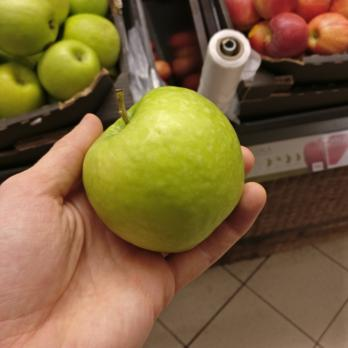
\includegraphics[width=30pt]{Chapter1/pics_paperA/Granny-Smith_021.jpg}}};
				\end{scope}
				\begin{scope}[xshift=34pt]
					\node {\fbox{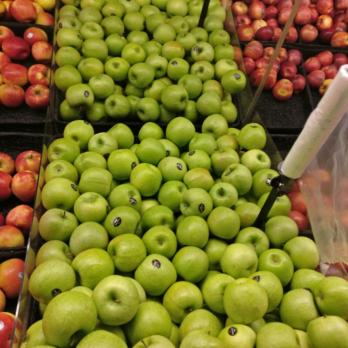
\includegraphics[width=30pt]{Chapter1/pics_paperA/Granny-Smith_012.jpg}}};
				\end{scope}
		\end{tikzpicture} }& 
		\makecell{\begin{tikzpicture}
				\begin{scope}
					\node {\fbox{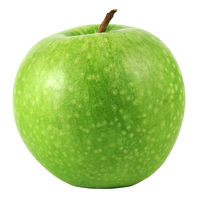
\includegraphics[width=30pt]{Chapter1/pics_paperA/Granny-Smith_Iconic.jpg}}};
				\end{scope}
		\end{tikzpicture} } & 
		\begin{scriptsize}
			\makecell{ \textit{“...\textbf{green} apple with \textbf{white, firm} pulp } \\[-1pt]  \textit{and a \textbf{clear acidity} in the flavor.”} } 
		\end{scriptsize}
		\\
		\hline 
		\makecell{ \scriptsize Tropicana \\[-1pt] \scriptsize Mandarin \\[-1pt] \scriptsize (Juice)}
		&  \makecell{ \begin{tikzpicture}
				\begin{scope}
					\node {\fbox{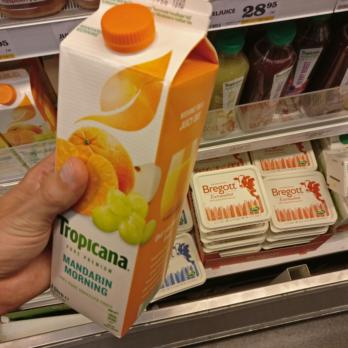
\includegraphics[width=30pt]{Chapter1/pics_paperA/Tropicana-Mandarin-Morning_003.jpg}}};
				\end{scope}
				\begin{scope}[xshift=34pt]
					\node {\fbox{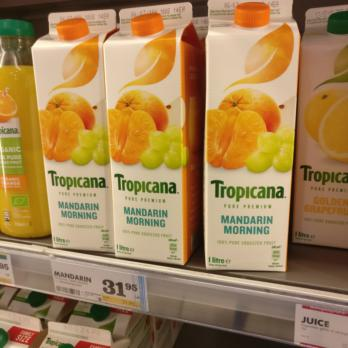
\includegraphics[width=30pt]{Chapter1/pics_paperA/Tropicana-Mandarin-Morning_016.jpg}}};
				\end{scope}
		\end{tikzpicture} }& 
		\makecell{\begin{tikzpicture}
				\begin{scope}
					\node {\fbox{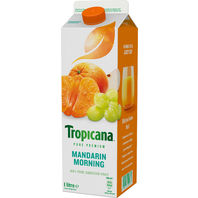
\includegraphics[width=30pt]{Chapter1/pics_paperA/Tropicana-Mandarin-Morning_Iconic.jpg}}};
				\end{scope}
		\end{tikzpicture} } & 
		\begin{scriptsize}
			\makecell{ \textit{“…is a \textbf{ready to drink} juice} \\[-1pt]
				\textit{\textbf{without pulp} pressed on \textbf{orange},} \\[-1pt]
				\textit{ \textbf{mandarin} and \textbf{grapes}. Not from} \\[-1pt]
				\textit{concentrate. Mildly \textbf{pasteurized}.” } }
		\end{scriptsize}
		\\
		\hline
	\end{tabular}
	%}
	}
	\label{tab:paperA}
	\vspace{-2mm}
\end{table}


\begin{enumerate}
	\item[] \textbf{Marcus Klasson}, Cheng Zhang, Hedvig Kjellström. In \textit{IEEE Winter Conference on Applications of Computer Vision (WACV) 2019}.
\end{enumerate}

\vspace{-3mm}
\paragraph{Summary:} We collect a dataset with natural images of raw and refrigerated grocery items taken in grocery stores in Stockholm, Sweden, for evaluating image classifiers on a challenging real-world scenario. The data collection was performed by taking photos of groceries with a mobile phone to simulate a scenario of grocery shopping using an assistive vision app. Furthermore, we downloaded iconic images and text descriptions of each grocery item by web-scraping a grocery store website to enhance the dataset with information describing the semantics of each individual item. The items are grouped based on their type, e.g., apple, juice, etc., to provide the dataset with a hierarchical labeling structure. We show two examples of grocery item classes and their corresponding web-scraped information in Table \ref{tab:paperA}. We provide benchmark results evaluated using pre-trained and fine-tuned convolutional networks for image classification.

\vspace{-3mm}
\paragraph{Author Contributions:}
CZ and HK presented the idea and the data collection procedure for the natural images and web-scraped information. MK performed the data collection including visiting the grocery stores for taking the natural images and the web-scraping of the grocery store website for iconic images and text descriptions. MK performed all the experiments and wrote most of the text. All authors took part in discussing the results and contributed to writing the manuscript. 


\subsection{\underline{Paper B}: Using Variational Multi-View Learning for Classification of Grocery Items}

%Visualizations of the latent representations from the test set, where we plot the iconic image of the corresponding object classes. We also plot the PCA projection of the natural image features from the off-the-shelf DenseNet169 in Figure \ref{fig:pca_densenet}. All models have been initialized with the same random seed before training. Abbreviations: VAE, Variational Autoencoder; VCCA, Variational Canonical Correlation Analysis.

%Visualizations of the latent representations $\mu_{z}$ of the red and green apples in the Grocery Store dataset. The red points correspond to the red apple classes, while the green points correspond to the green apple. The blue points correspond to the other grocery items. Abbreviations: VCCA, Variational Canonical Correlation Analysis.

\begin{enumerate}
	\item[] \textbf{Marcus Klasson}, Cheng Zhang, Hedvig Kjellström. In \textit{Patterns, Volume 1(8) (2020)}.
\end{enumerate}

\vspace{-3mm}
\begin{wrapfigure}[14]{r}[-4mm]{0.5\textwidth}
	\centering
	\vspace{-5mm}
	\begin{subfigure}[b]{0.26\textwidth}
		\centering
		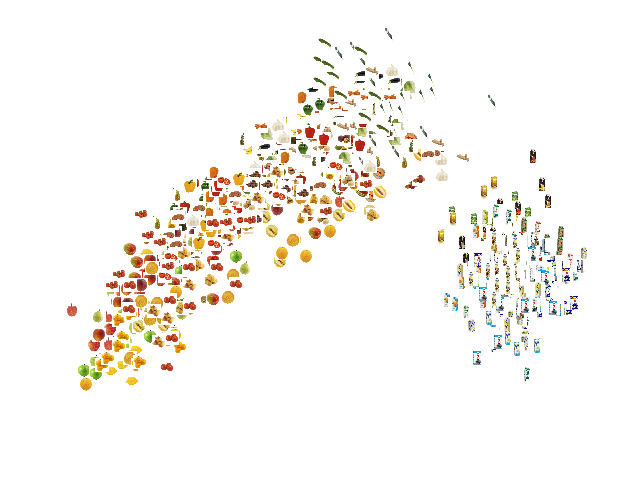
\includegraphics[width=\textwidth]{Chapter1/pics_paperB/pca_latents_vae_seed2}
		\vspace{-7mm}
		\caption{VAE$_{\vx}$}
		\label{fig:pca_latents_vae}
	\end{subfigure} 
	\hspace{-5mm}
	%\hfill
	\begin{subfigure}[b]{0.26\textwidth}
		\centering
		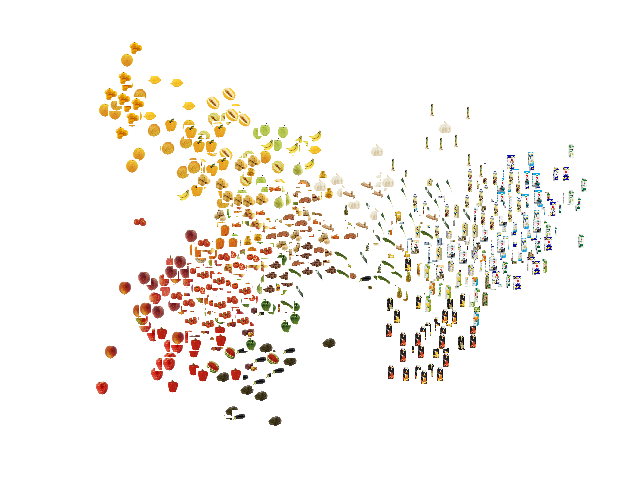
\includegraphics[width=\textwidth]{Chapter1/pics_paperB/pca_latents_vcca_xiwy_seed2}
		\vspace{-7mm}
		\caption{VCCA$_{\vx \vi \vw \vy}$ }
		\label{fig:pca_latents_vcca_xiwy}
	\end{subfigure}
	\vspace{-6mm}
	\captionsetup{width=.46\textwidth}
	\caption{Visualizations of the latent representations projected in 2D space with PCA from models VAE$_{\vx}$ and VCCA$_{\vx \vi \vw \vy}$, where we plot the corresponding iconic image for each latent representation. We observe that VCCA$_{\vx \vi \vw \vy}$ structures the items based on visual similarities by incorporating the web-scraped information into the learning. 
	}
	%\vspace{-3mm}
	\label{fig:paperB_pca_latents}
\end{wrapfigure} 
\paragraph{Summary:} 
We investigate whether training image classifiers benefits from combining the natural images and web-scraped information in the Grocery Store dataset from Paper \ref{paperA}. We employ a deep generative model called Variational Canonical Correlation Analysis (VCCA)~\cite{wang2016deep} for learning joint representations of the different data views, i.e., natural images, iconic images, and text descriptions, that are used for training the classifiers. We performed a thorough ablation study over all data views to demonstrate how they contribute individually to enhancing the classification performance. Our results show that the iconic images help to group the items based on their color and shape while text descriptions separate the items based on differences in ingredients and flavor. Figure \ref{fig:paperB_pca_latents} shows visualizations of the latent representations learned by a variational autoencoder (VAE)~\cite{kingma2013auto} and VCCA. Finally, we concluded that utilizing the iconic images and text descriptions yielded better classification results than only using natural images. 

\vspace{-3mm}
\paragraph{Author Contributions:} CZ and HK presented the idea and all authors contributed to formalizing the methodology. MK performed all the experiments, created the visualizations, and wrote most of the text. All authors took part in discussing the results and contributed to writing the manuscript. 



\subsection{\underline{Paper C}: Learn the Time to Learn: Replay Scheduling for Continual Learning}

\begin{figure}[t]
	\centering 
    \begin{subfigure}[b]{0.48\textwidth}
		\centering
		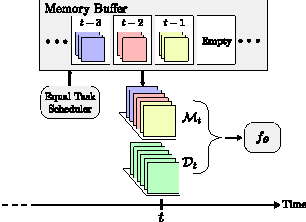
\includegraphics[width=\textwidth]{Chapter1/figures/replay_approach_new.pdf}
		\caption{The traditional replay approach.}
		\label{fig:paperC_standard_replay}
	\end{subfigure}~
    \begin{subfigure}[b]{0.48\textwidth}
		\centering
		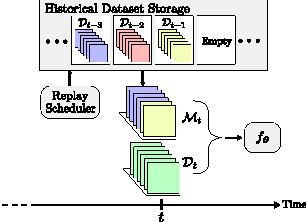
\includegraphics[width=\textwidth]{Chapter1/figures/replay_scheduling_new.pdf}
		\caption{Our replay scheduling approach.}
		\label{fig:paperC_our_approach}
	\end{subfigure}
	%\includegraphics[width=0.33\textwidth]{example-image-c}
	\caption{Illustrations of the (a) traditional replay approach where an equal amount of old samples in a small memory buffer are replayed at every time, and (b) our replay scheduling approach from Paper \ref{paperC} where the scheduler selects which tasks to replay by selecting samples from the stored previously seen datasets.}
	\vspace{-2mm}
	\label{fig:paperC}
\end{figure}

\begin{enumerate}
	\item[] \textbf{Marcus Klasson}, Hedvig Kjellström, Cheng Zhang. \textit{Unpublished manuscript}. %Submitted to \textit{International Conference on Machine Learning (ICML) 2022}.
\end{enumerate}

\vspace{-3mm}
\paragraph{Summary:} We present a slightly altered CL setting where the historical data is accessible at any time to mitigate catastrophic forgetting. However, retraining the CL system from all historical data is prohibitive due to constraints on processing times. To this end, we propose to learn the time to learn for a CL system, in which we learn schedules over which tasks to replay at different times. Figure \ref{fig:paperC} illustrates the differences between our replay scheduling approach and the traditional replay approach in CL. We study the benefits of replay scheduling by allowing multiple episodes in the CL environment to enable searches for efficient replay schedules using Monte Carlo tree search. We show that the replay schedules from MCTS can significantly improve the performance compared to baselines with scheduling policies. We conclude that learning the time to replay different tasks can be critical for the performance of replay-based methods in our new proposed CL setting. 

\vspace{-3mm}
\paragraph{Author Contributions:} CZ presented the idea, and MK and CZ contributed to formalizing the methodology. MK performed all the experiments, created the visualizations, and wrote the text. All authors took part in discussing the results and contributed to writing the manuscript. 


\subsection{\underline{Paper D}: %Meta 
	Policy Learning for Replay Scheduling in Continual Learning}


\begin{enumerate}
	\item[] \textbf{Marcus Klasson}, Hedvig Kjellström, Cheng Zhang. \textit{Unpublished manuscript}.%Under preparation for submission to \textit{Conference on Neural Information Processing Systems (NeurIPS) 2022}.
\end{enumerate}


\vspace{-3mm}
\paragraph{Summary:} To enable replay scheduling in real-world CL scenarios, we propose a reinforcement learning-based framework for learning replay scheduling policies. Figure \ref{fig:paperD_our_approach} illustrates the pipeline of our framework. Our intuition is that there may exist general patterns regarding the replay scheduling, e.g., tasks that are harder or have been forgotten should be replayed more often. Therefore, we define the state as the validation performance of the classifier, which is passed to the policy that selects actions for how to compose the replay memory to efficiently mitigate catastrophic forgetting. Our framework enables learning policies that can generalize to new CL scenarios without additional computational cost or training in the test environment. In the experiments, we show that the learned policies can generalize to CL scenarios with new task orders and datasets unseen during training. 

\vspace{-3mm}
\paragraph{Author Contributions:} CZ presented the idea, and MK and CZ contributed to formalizing the methodology. MK performed all the experiments, created the visualizations, and wrote most of the text. All authors took part in discussing the results and contributed to writing the manuscript. 

\begin{figure}[t]
	\centering 
	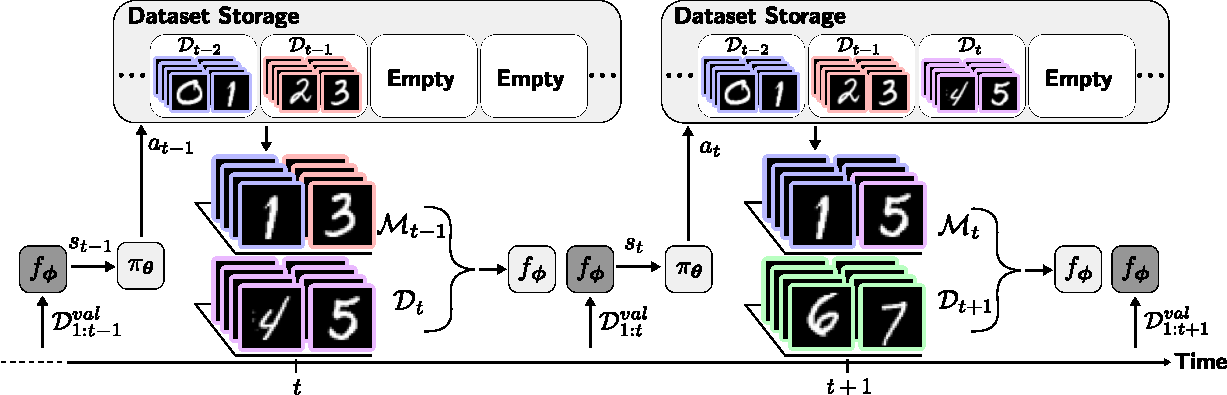
\includegraphics[width=0.95\textwidth]{Chapter1/figures/testing_size2.pdf}
	\caption{Illustration over our policy learning framework for replay scheduling prposed in Paper \ref{paperD}. The policy $\pi_{\vtheta}$ receives state $s_t$ of the classifier $f_{\vphi}$ to select action $a_t$ determining how the replay memory $\gM_t$ should be constructed. Dark gray-shaded box means that classifier is in evaluation mode.}
	\label{fig:paperD_our_approach}
	\vspace{-2mm}
\end{figure}

% Thesis outline
\section{Thesis Outline}\label{chap1:sec:outline}
The rest of the thesis is organized as follows: Chapter \ref{chap2} provides some preliminaries on deep learning methods in computer vision that we used in this thesis. Chapter \ref{chap3} is focused on our contributions in FGIR where we summarize Paper \ref{paperA} and \ref{paperB} on grocery item classification with an assistive vision app. Similarly, in Chapter \ref{chap4}, we focus on our contributions in CL and summarize the content in Paper \ref{paperC} and \ref{paperD} on our proposed replay scheduling approach in CL. Finally, in Chapter \ref{chap5}, we provide our conclusions of the presented works and present some potential research directions that we believe could be interesting to look deeper into in future research on computer vision-based assistive technologies. 
